\chapter{Modular Programming in Squeak}
\label{sec:problem}
In this section, we describe and evaluate how Squeak can be used to write modular programs at the moment. Based on our observations and programming experience with Squeak, there are three areas where we see room for improvement. For every area, we will describe what the problem is and how it is currently solved in Squeak.

\paragraph{Class-based Modularity}
In pure Smalltalk, classes are the highest level of modular units. Classes are first-class objects and can be passed around. This functionality can be used to make behavior interchangable and promotes loose coupling. Classes are Smalltalk's way of sharing behavior with a number of objects, i.e., it is a form of code reuse. Squeak also supports Traits, a design method for composing classes out of pieces of behavior (see Section~\ref{sec:rel_traits}).

Smalltalk is, as most object-oriented and class-based programming languages, amenable to well-established software design patterns~\cite{Gamma:1995:DPE:186897}, making it easier to write maintainable and understandable code.

\section{Duplicate Class Names}
In Squeak, there can be only one class with a certain name, limiting code reuse and, therefore, hindering modular composability. Whenever the programmer tries to add another class with the same name, a conflict occurs. When source code is loaded into the system with the Monticello source control system or manually, the system asks the programmer if the already existing class should be replaced. As a workaround, it is good practice to add unique namespace prefixes to all class names within an application. 

Squeak has packages~\cite{Nierstrasz:2009:SE:1816759}, but these are not used as namespaces. Their purpose is to make it easier to find existing classes (like method protocols). They are also used as deployment units. The programmer does usually not load single classes into the system. Instead, packages (groups of classes) are loaded. 

Squeak environments provide a way to have multiple classes with the same name in one image. However, they suffer from poor tooling and do not integrate well with some of the other goals for our system. See Section~\ref{sec:rel_sq_env} for a detailed discussion of Squeak environments and why we did not use them in \msname.

\paragraph{Example}
\begin{figure}[!htp]
\dirtree{%
.1 \framebox{\textbf{BroBreakout}}.
.2 BroBall.
.2 BroBlock.
.2 BroBoundary.
.2 BroBreakout.
.2 BroExplosion.
.2 BroLevelBuilder.
.2 BroLevelStatistics.
.2 BroLevelStatisticsItem.
.2 BroLevelView.
.2 BroLevelWorld.
.2 BroMenuLabel.
.2 BroMenuView.
.2 \textit{BroPowerup}.
.2 BroPowerupAccelerate.
.2 BroPowerupBall.
.2 BroPowerupDecelerate.
.2 BroPowerupEnlarge.
.2 BroPowerupShrink.
.2 BroRacket.
.2 \textit{BroView}.
.2 BroWelcomeView.
}
\caption[Example: Breakout class structure]{Example: Breakout class structure. All classes have the \texttt{Bro} namespace prefix and are contained in the package \texttt{BroBreakout}.}
\label{fig:conc_breakout}
\end{figure}

Consider the game Breakout (Figure~\ref{fig:conc_breakout}, see also Section~\ref{sec:usecase_hierach_decomp}). This application uses \texttt{Bro} as a prefix for all classes. If we would not use namespace prefixes, generic class names like \texttt{Block} or \texttt{Ball} would be likely to collide with other classes. On the other hand, if all application and library developers adhere to this convention, it is unlikely that class name clashes occur.

\section{Dependency Managment}
Dependency management describes the task of keeping track of dependencies and ensuring that required dependencies are available within the application/library in question. We distinguish between two cases of dependency management: internal dependency management, i.e., the application specifies all dependencies, and external dependency managment (\emph{external configuration}), i.e., users/clients of the application specify dependencies. But before managing dependencies, we need a versioning concept that allows us to represent library versions in an image.

\paragraph{Versioning}

There are situations when it is useful to have multiple versions of the same library in one image; for example, if there are two different applications installed and both require the same library, but in different versions~\cite{springerniephaus}. Consider, for example, that application \emph{A} requires two libraries \emph{B} and \emph{C}, both of which require dependency \emph{D}, but in different versions (Figure~\ref{fig:concept_problem}), which is called a \emph{transitive dependency version conflict}. \emph{B} requires \emph{D} in version 1.1 and \emph{C} requires \emph{D} in version 3.2. Both \emph{B} and \emph{C} might function properly with version 3.2 of \emph{D} if \emph{D}'s interface and behavior have not changed. However, we do usually not know this in advance, and especially with new major versions, interfaces tend to change. Old versions of a library might have bugs that an application has to work around. An application might then not work with a newer library, where the bug is fixed.

\begin{wrapfigure}{l}{0.5\textwidth}
	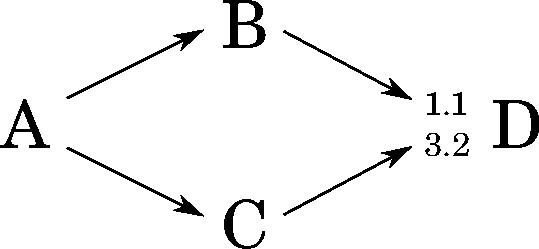
\includegraphics[scale=0.65]{concept_problem.pdf}
	\centering
	\caption[Example: Transitive dependency version conflict]{Example: Transitive dependency version conflict. Two different versions of \emph{D} are required for running \emph{A}.}
	\label{fig:concept_problem}
\end{wrapfigure}

Therefore, we need a versioning mechanism in \msname, that helps us storing and referencing different versions of the same application or library in one image. Part of this mechanism must be a way to develop new library versions, and a mechanism to reference a certain version.

\paragraph{Internal Dependency Management}
In this case, every application or library specifies itself which dependencies (and their versions) it depends on. The application effectively maintains the list of dependencies itself. Consequently, the application is coupled with its dependencies and cannot be used with different versions or implementations without changing its source code.

A form of internal dependency managment is \emph{dependency injection}, a mechanism that is heavily used in the Java world~\cite{Prasanna:2009:DI:1795686}. What a class specifies is that it requires \emph{some} dependency implementing a certain interface, but not what exact dependency it is or in what version. Dependency injection is also known as \emph{inversion of control}~\cite{fowlerioc}, because it inverts the control of dependencies: it is shifted from the classes using a dependency to the \emph{injector}, a component that is usually part of the application and knows about all dependencies. The benefit of this approach is that all dependencies are managed at a central position in the application.

\paragraph{External Configuration}
In this case, the dependency management is delegated to the client/user of an application or library. What the application specifies is that it requires some dependency implementing a certain interface, but not what exact dependency it is or in what version. Conrete dependencies are provided by the client. External configuration is useful for dependencies with variation points, i.e., modules that can be used with different dependencies, based on the use case. For example, an application might want to use a graph library with an adjacency list instead of an adjacency matrix data structure, if it operates on sparse graphs; both implement the same interface. Another example is an image editing library that needs \emph{some} dependency for exporting images to the file system, but it is up to the client to decide which file format to use. 

External configuration is beneficial for modularity, because it supports loose coupling of applications and dependencies. This, in turn, promotes understandability, maintainablity, and exchangability (code reuse), because an application cannot rely on implementation details of a loosely bound dependency.

\paragraph{Dependency Management in Squeak}
In Squeak, there can currently only be one version of a library or application installed at a time. Monticello is used as a source code management system and loads new versions of the source code into an image. Metacello is a package management system (see Section~\ref{sec:rel_metacello}), similar to Maven in Java. Every Metacello package has a configuration class containing a list of external dependencies and internal packages to load for every version, along with the location of an external repository where the packages should be loaded from~\cite{metacellodraft}.

External configuration can be simulated in Smalltalk by writing class constructors that accept other dependencies as parameters. These dependencies should then be stored in instance variables and only be accessed using these instance variables. However, this technique has two pitfalls. Firstly, dependencies have to be forwarded to all other classes, resulting in boilerplate code. Secondly, only instance methods can benefit from external configuration, because class methods are shared among instances (configurations) of the class and do not have access to instance variables.

\msname needs a structured way to reference dependencies. The source code should not be filled with references to external dependencies. It should be easy to replace one dependency with another one or to change the version number of a dependent module. Furthermore, running two applications requiring he same library in different versions in one image should not be a problem.

\section{Hierarchical Decomposition}
\label{sec:problem_hier_decomp}
Smalltalk packages allow the programmer to group together what belongs together~\cite{Eckel:2002:TJ:579108}. This is especially useful in big projects with many classes and allows for a form of modular decomposition. Different criterias for modular decomposition have been proposed: e.g., functional decompositon (making every step in the \emph{flowchart} a module) or information hiding~\cite{Parnas:1972:CUD:361598.361623, Parnas:1984:MSC:800054.801999}. The following list shows some benefits of good modular decomposition.

\begin{itemize}
	\item Changability (continuity): only few classes are affected when changing a detail.
	\item Independent development: classes can be developed in parallel.
	\item Understandability: in order to understand the behavior of a class, it is sufficient to read code within that class.
\end{itemize}

What we want to achieve is hierarchical decomposition~\cite{Blume:1999:HM:325478.325518}, which is in a basic form realized in Java packages, Ruby namespace modules, or Python modules. It can increase comprehensibility of the overall system when it acts as some kind of decision tree that helps the programmer finding a submodule corresponding to a certain functionality in an unknown application. 

%It also allows for fine-grained dependency management: for example, it is considered good practice in many programming languages to keep import statements as small as possible. Import statements also act as documentation, giving the reader of the source code a rough idea of what the source code might do. Furthermore, if a functionality is nested in a submodule, it is likely that it is written in a more general way, such that it might be reused elsewhere in the application without bigger changes.

If the source code is functionally decomposed in a hierarchical way~\cite{Tsui:2009:ESE:1823101}, it is also easier to understand single submodules of the system. The reader of the source code might only be interested in a certain level of detail (e.g., no low-level functionality), and then skip deeply nested submodules~\cite{hierarch1} (information hiding or abstraction). Since in functional decomposition, the purpose of nested modules is usually only to serve their enclosing modules, readers can start off with a high-level idea of what the module is doing by going through the first few levels of nesting, and dive in deeper as needed.

Therefore, one of the requirements for our system is to provide a mechanism for hierarchical code decomposition that is more than just one level deep (Smalltalk packages).

\paragraph{Example}
Consider the game SpaceCleanup, which is a simple bomberman clone (Figure~\ref{fig:prob_space_cleanup_org}, see also Section~\ref{sec:usecase_hierach_decomp}). The source code for this game is organized in multiple packages. For example, all items in the game are grouped in the package \texttt{SpaceCleanup-Items}. Besides this obvious single-level decomposition, the game is actually already functionally decomposed in a hierarchical way. For example, \texttt{ScuLevel} represents a level in the game. A level consists of multiple tiles (\texttt{ScuTile}). A tile cannot exist without a level; its sole purpose is to serve \texttt{ScuLevel}. Similarly, items always belong to a tile and cannot be used without a tile. All in all, SpaceCleanup is already functionally decomposed, but this decomposition is not fully reflected in the class organization.

\begin{figure}[!htp]
\dirtree{%
.1 \framebox{\textbf{SpaceCleanup-Core}}.
.2 ScuEventDispatcher.
.2 ScuGame.
.2 ScuGameBuildState.
.2 ScuGameConfigState.
.2 ScuGameOverState.
.2 ScuGamePausedState.
.2 ScuGameRunningState.
.2 \textit{ScuGameState}.
.2 ScuGameWonState.
.2 \textit{ScuMonsterStrategy}.
.2 ScuMonsterRandomStrategy.
.2 ScuMonsterToPlayerStrategy.
}
\vspace{10pt}
\dirtree{%
.1 \framebox{\textbf{SpaceCleanup-Items}}.
.2 ScuBucket.
.2 \textit{ScuDestructibleItem}.
.2 ScuFloor.
.2 \textit{ScuItem}.
.2 ScuMonster.
.2 \textit{ScuMovingItem}.
.2 ScuPickUpItem.
.2 ScuPlayer.
.2 ScuPortal.
.2 ScuSlime.
.2 ScuWall.
.2 ScuWater.
}
\vspace{10pt}
\dirtree{%
.1 \framebox{\textbf{SpaceCleanup-Level}}.
.2 ScuLevel.
.2 \textit{ScuLevelBuilder}.
.2 ScuGridPatternLevelBuilder.
.2 ScuRandomLevelBuilder.
.2 ScuTile.
}
\vspace{10pt}
\dirtree{%
.1 \framebox{\textbf{SpaceCleanup-Resources}}.
.2 ScuResourceManager.
}
\vspace{10pt}
\dirtree{%
.1 \framebox{\textbf{SpaceCleanup-UI}}.
.2 ScuCheatWindow.
.2 ScuConfigurationWindow.
.2 ScuControls.
.2 ScuGameInformation.
}
\caption[Example: SpaceCleanup class organization]{Example: SpaceCleanup class organization. All classes have the \texttt{Scu} namespace prefix and are grouped in five packages, according to their responsibilities.}
\label{fig:prob_space_cleanup_org}
\end{figure}


%\section{Code Reuse}
%share behavior among multiple classes
